
\chapter{Background}
\label{chap:back}

This chapter presents a briefly theoretical background as to mathematical tools and basics of computer vision. In addition, the API and tools used in this thesis. To dive deeply in any topic described ahead, a reference is given.


\section{ Mathematical Tools}
\subsection{Rigid Transformations}\label{rigidtf0}
A rigid transformation also called Euclidean transformation is a geometric transformation of a Euclidean space that preserves the Euclidean distance between every pair of points. The rigid transformations include rotations, translations, reflections, or their combination. It can be shown that all rigid transformations can be expressed as follows.

\begin{equation}\label{rigidtf}
 g_(v)=R \cdot v + t, R \in \mathbb{R}^{3}
\end{equation}

A rigid transformation can be represented by using $4x4$ matrices by employing a homogenous coordinates as follows:
$$
\begin{pmatrix}
R & t \\
0 & 1
\end{pmatrix}
\begin{pmatrix}
P \\
1
\end{pmatrix}=
\begin{pmatrix}
RP+t \\
1
\end{pmatrix}
$$

 In the equation \ref{rigidtf} the matrix, R, is referred to as a rotation matrix and has the following special properties.
\begin{itemize}
\item $R=(a\,  b\,  c), \, a,b,c \in \mathbb{R}^{3}$
\item $\|a\|=\|b\|=\|c\|=1 $ All columns are unit length
\item $a \cdot b=b \cdot c=c \cdot a=0 $ The columns are mutually orthogonal
\end{itemize}
\subsection{Rotation Matrices}
The matrix R, a set of 3x3 matrices with the following properties, plus the operation of matrix multiplication forms a group called SO(3) which stands for special orthogonal group $\in \mathbb{R}^{3} $

$R=(a\,  b\,  c), \, a,b,c \in \mathbb{R}^{3}$ is a rotation matrix for $\mathbb{R}^{3}$ iff
\begin{itemize}
\item $R^{T} \cdot R=I$
\item $det(R)=1$
\end{itemize}

\subsubsection{Rotation Representations}
\begin{itemize}
\item A rotation can be expressed as a $3X3$ matrix $R \in SO(3)$  where $R^{T} \cdot R= R \cdot R^{T} =I$ and $det(R)=1$

\item A rotation can also be expressed in terms of an angle $\theta$  and an axix $\hat{\omega} \in \mathbb{R}^{3}$ where $\|\hat{\omega}\|=1$. It can relate to the matrix form via the Rodrigues formula.
$$R=exp(\theta J(\omega))=I+\sin \theta J(\omega)+(1-\cos \theta)J(\hat{\omega})^{2}$$

\item And finally a rotation matrix expressed as a unit quaternion:
$$(u_{0},u)=(\cos(\frac{\theta}{2}),\sin(\frac{\theta}{2})\hat{\omega})$$
\end{itemize}


\section{Basics of 3D Computer Vision}
\subsection{ RGB-D sensors} \label{rgbdcamera}
Nowadays novel camera systems like the Astra Orbbec and RealSense which provide both color and depth images have become readily available. Therefore, there are great expectations that such sensory devices will lead to a boost of new 3D perception-based applications in the fields of robotics. We are specifically interested in using RGB-D sensors for recognition and localization of an isolated part. In this thesis, both cameras are used. See Figure \ref{fig:mycam} in order to be acquainted with them.

\begin{figure}%
    \centering
    \subfloat[Astra Camera]{{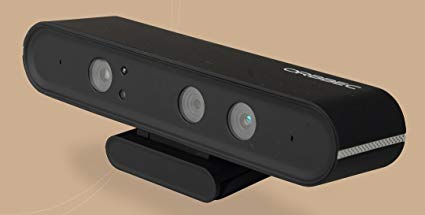
\includegraphics[width=5cm]{figures02/astraorbbec.jpg} }}%
    \qquad
    \subfloat[RealSense Camera]{{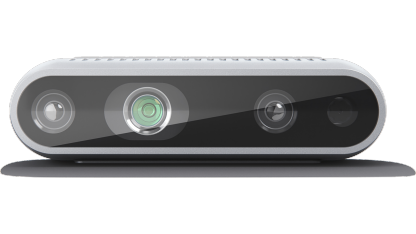
\includegraphics[width=5cm]{figures02/realsense.png} }}%
    \caption{2 RGB-D sensors}%
    \label{fig:mycam}%
\end{figure}

\iffalse
\begin{figure}[!h]
\begin{center}
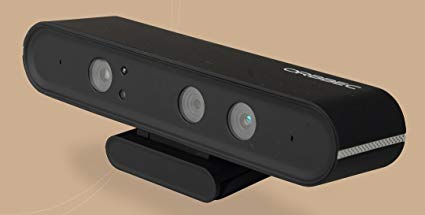
\includegraphics[width=2in]{figures02/astraorbbec.jpg}
\caption{RGB-D sensor(from Astra Orbbec documentation))}%\cite{temp2}}
\end{center}
%\label{fig2:mypicture3}
\end{figure}
\fi

\subsubsection{Point Cloud}

 The receive measurement data from the input sensor get converted in a more generic data structure called point cloud, which is a set of vertices in a three-dimensional coordinate system usually defined by X, Y, and Z coordinates. The vertices are typically intended to represent the external surface of an object.
 Point clouds can be acquired from hardware sensors such as stereo cameras, 3D scanners, or time-of-flight cameras, or generated from a computer program synthetically. In this thesis, the point cloud is acquired from the sensory devices briefly described above in \ref{rgbdcamera}.


\begin{figure}[!h]
\begin{center}
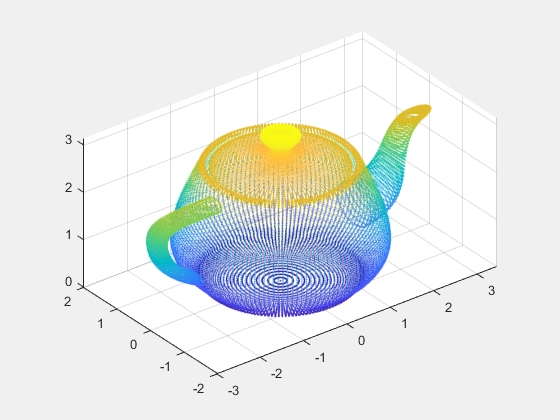
\includegraphics[width=4in]{figures02/pcd.png}
\caption{Overview of a point cloud (from MathWorks documentation)}%\cite{temp2}}
\end{center}
\label{fig2:mypicture3}
\end{figure}


\subsection{ Camera Pinhole Model}\label{pinhole}
There are many lens models but Pinhole camera is used in this thesis. A pinhole camera is the simplest model that captures accurately the geometry of perspective projection. The image of the object is formed by the intersection of the light rays with the image plane. An illustration of the pinhole camera is seen in  Figure 1. This mapping from the three dimensions onto two dimensions is called perspective projection. The camera projects point in the world frame $ P_{w}=(X,Y,Z)^{T} \in \textbf{R}^{3}$ through the pinhole to  the point $p_{c}=(u,v)$ on the image plane.
 
\begin{figure}[!h]
\begin{center}
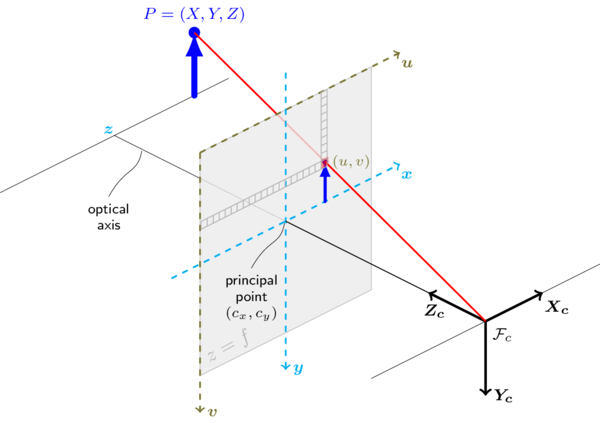
\includegraphics[width=2in]{figures02/pinhole_camera_model.png}
\caption{View of a Pinhole camera geometry (from Camera Calibration and 3D Reconstruction, openCV)}%\cite{temp2}}
\end{center}
%\label{fig2:mypicture3}
\end{figure}

\subsection{Parameters of camera model}
We use $(u,v,1)^{T}$ to represent a 2D point position in pixel coordinates or image plane. And $(x_{w},y_{w},z_{w},1)^{T}$ is used to represent a 3D point position in world coordinates. Note: they were expressed in augmented notation of homogeneous coordinates which is the most common notation in robotics and rigid body transforms. Referring to the pinhole camera model, a camera matrix is used to denote a projective mapping from world coordinates  to Pixel coordinates(or image plane), the camera matrix is giving by Eq. \ref{eq1}.

\begin{equation}\label{eq1}
z_{c}*
\left[ {\begin{array}{c}
u \\
v \\
1 \\
\end{array} } \right]
= K*
\left[ {\begin{array}{c}
\textbf{R} \ \textbf{t} \\
\end{array} } \right]
*\left[ {\begin{array}{c}
X_{w}\\
Y_{w} \\
Z_{w} \\
1\\
\end{array} } \right]\end{equation}

\subsection{Camera's Intrinsic Parameters}
Images coordinates are measured in pixels, normally with the origin in the left upper corner. The focal
plane in the pinhole camera model is embedded $\in R^{3}$ so we need to have a mapping that translates
the points in the image plane into pixels, see Figure \ref{fig:intrinsic}.

\begin{equation}\label{eq2}
   K=
    \left[ {\begin{array}{cccc}
   f_{x} & 0 & c_{x} \\
   0 & f_{y} & c_{y} \\
   0 & 0 & 1\\

  \end{array} } \right]    
\end{equation}



\begin{figure}[!h]
\begin{center}
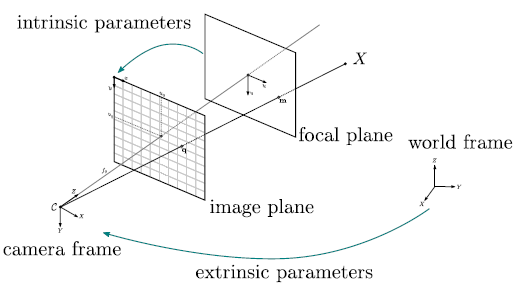
\includegraphics[width=4in]{figures02/intrinsic.png}
\caption{Overview of the transformation between the focal plane and the image plane}%\cite{temp2}}
\label{fig:intrinsic}
\end{center}
\end{figure}


\subsection{Camera's Extrinsic Parameters}

The transformation between the world coordinate system and the camera coordinate system is achieved be a rotation and a translation. The translation is represented by a vector $t \in \textbf{R}^{3}$ and the rotation by a 3x3 orthogonal matrix \textbf{R}. So $\textbf{R}$ represents a rotation matrix, and it must satisfy the following properties:

\begin{equation}\label{eq3} 
     det(\textbf{R})=1 
\end{equation}
\begin{equation}\label{eq4}  
    \textbf{R}^{T}\textbf{R}=I      
\end{equation}


Where I is the identity matrix. The matrix \textbf{R} and the vector \textbf{t} altogether are called camera's extrinsic parameters, see Figure.

\begin{figure}[!h]
\begin{center}
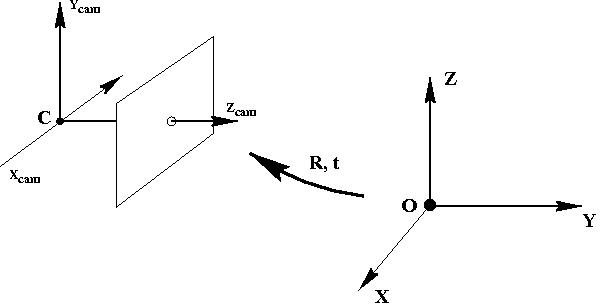
\includegraphics[width=4in]{figures02/extrinsic.png}
\caption{Overview of a world coordinate system and camera coordinate system}%\cite{temp2}}
\end{center}
%\label{fig2:mypicture3}
\end{figure}


The transformation of a representation of point in the world coordinate system, $ P_{w}=(X,Y,Z)^{T}$ into the camera coordinate system, $ P_{c}=(X,Y,Z)^{T}$ can be done with the following equation.
\begin{equation}\label{eq4} 
P_{c}=\textbf{R}.P_{w}+\textbf{t}
\end{equation}

 The Equation \ref{eq4} can also be written as:


\begin{equation}\label{eq5} 
    P_{c}=\left[\textbf{R} \ \textbf{t}\right]\left[\frac{P_{w}}{1}\right]   
\end{equation}

\section{Robotic Operating System}

For this thesis The Robotic Operating System (ROS) is used as main platform. In addition, it is used for visualization purpose and debugging steps. ROS is a flexible framework for writing robot software. In addition, it is  a collection of tools, libraries, and conventions that aim to simplify the task of creating complex and robust robot behaviour across a wide variety of robotic platforms. It is based on the concepts of nodes, topics, messages and services. A node is an executable program that performs computation. Nodes need to communicate with each other to complete the whole task. The communicated data are called messages. ROS provides an easy way for passing messages and establishing communication links between nodes, which are running independently. They pass these messages to each other over a Topic, which is a simple string, Topics are asynchronous communication. As to, a synchronous communication, it is provided by services. Services act in a call-response manner where one node requests that another node execute a one-time computation and provide a response. For more details about ROS, the reader can refer to \cite{ros}.

\begin{figure}[!h]
\begin{center}
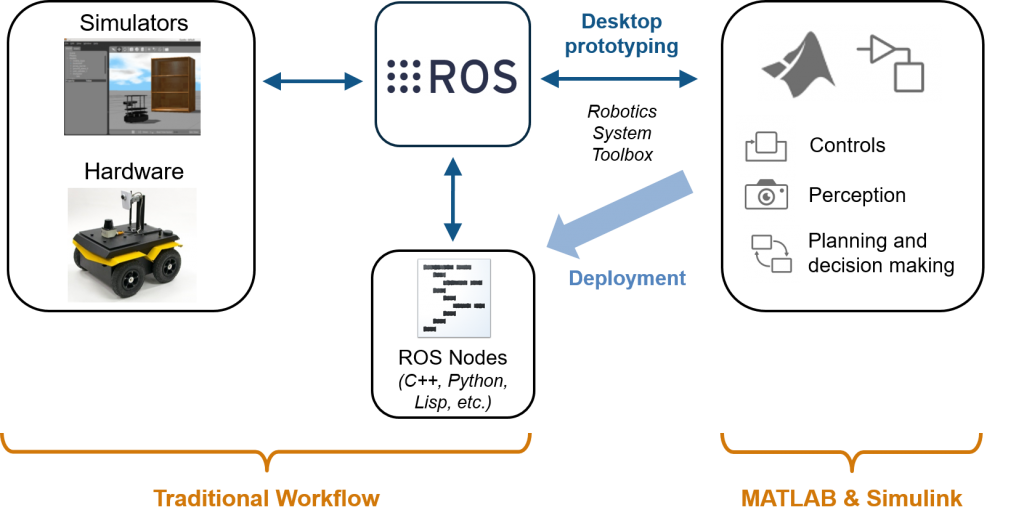
\includegraphics[width=4in]{figures02/ros_workflows.png}
\caption{A ROS Overview}%\cite{temp2}}
\end{center}
%\label{fig2:mypicture3}
\end{figure}

\section{Open-source Libraries}
\subsection{PCL}

The PCL\cite{pcl} framework contains numerous state-of-the art algorithms including filtering, feature estimation, surface reconstruction, registration, model fitting and segmentation. These algorithms can be used, for example, to filter outliers from noisy data, align 3D point clouds together, segment relevant parts of a scene, extract keypoints and compute descriptors to recognize objects in the world based on their geometric appearance, and create surfaces from point clouds and visualize them. 

For different processing steps, a Python bindings for the Point Cloud Library (PCL) is used. This is a reasonable python binding to the point cloud library. At present the following features of PCL, using PointXYZ point clouds, are available;

\begin{enumerate}
    \item I/O and integration; saving and loading PCD (point cloud data) files
    \item segmentation
    \item sample consensus model fittting (RANSAC + others, cylinders, planes, common geometry)
    \item smoothing (median least squares)
    \item filtering (voxel grid downsampling, passthrough, statistical outlier removal)
    \item exporting, importing and analysing pointclouds with numpy
\end{enumerate}

\begin{figure}[!h]
\begin{center}
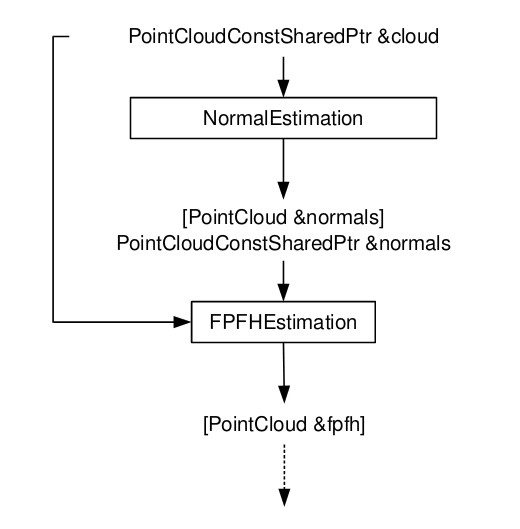
\includegraphics[width=4in]{figures02/pcl1.png}
\caption{An  example  of  the  PCL  implementation  pipeline  for  Fast  Point Feature Histogram (FPFH) \cite{fpfh} estimation.}
\end{center}
%\label{fig2:mypicture3}
\end{figure}


\subsection{Open3D}

For the purpose of working with any ideal registration algorithm, the Open3D is used in this thesis which is an open-source library that supports rapid development of software that deals with 3D data. The Open3D frontend exposes a set of carefully selected data structures and algorithms in both C++ and Python. Open3D provides data structures for three kinds of representations: point clouds, meshes, and RGB-D images.  For each representation, it offers a complete set of basic processing algorithms such as sampling, visualization, and data conversion. In addition, Open3D  provides  implementations  of  multiple  state-of-the-art surface registration methods, including pairwise global registration, pairwise local refinement as the ICP registration \cite{icp}, and multiway registration  using  pose  graph  optimization. 

\section{Software tools}
For the purpose of rendering, convertion and manipulation of any 3D data(CAD model) several tools from the open source communities are used in this thesis such as CloudCompare, MeshLab and FreeCAD. 

\subsection{CloudCompare}
CloudCompare is a 3D point cloud (and triangular mesh) processing software. It has been originally designed to perform comparison between two dense 3D points clouds (such as the ones acquired with a laser scanner) or between a point cloud and a triangular mesh. It relies on a specific octree structure dedicated to this task.  Afterwards, it has been extended to a more generic point cloud processing software, including many advanced algorithms (registration, resampling, color/normal/scalar fields handling, statistics computation, sensor management, interactive or automatic segmentation, display enhancement, etc.)\cite{cloudcompare},. 

\begin{figure}[!h]
\begin{center}
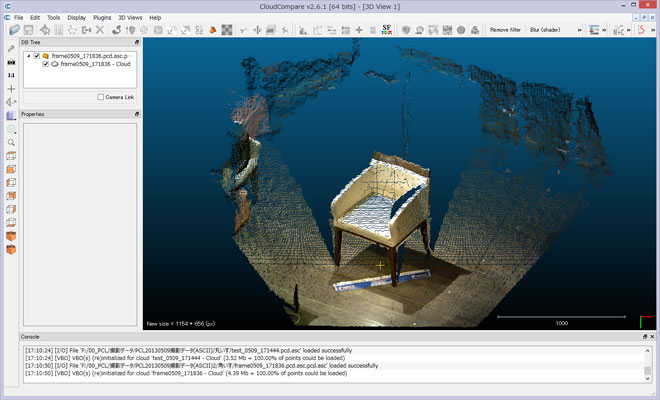
\includegraphics[width=4in]{figures02/cloudcompare.jpg}
\caption{CloudCompare (view, edit and process).}
\end{center}
%\label{fig2:mypicture3}
\end{figure}


\subsection{MeshLab}
Meshlab is an open source system for processing and editing 3D triangular meshes.
It provides a set of tools for editing, cleaning, healing, inspecting, rendering, texturing and converting meshes. It offers features for processing raw data produced by 3D digitization tools/devices and for preparing models for 3D printing \cite{meshlab}.

 \begin{figure}[!h]
\begin{center}
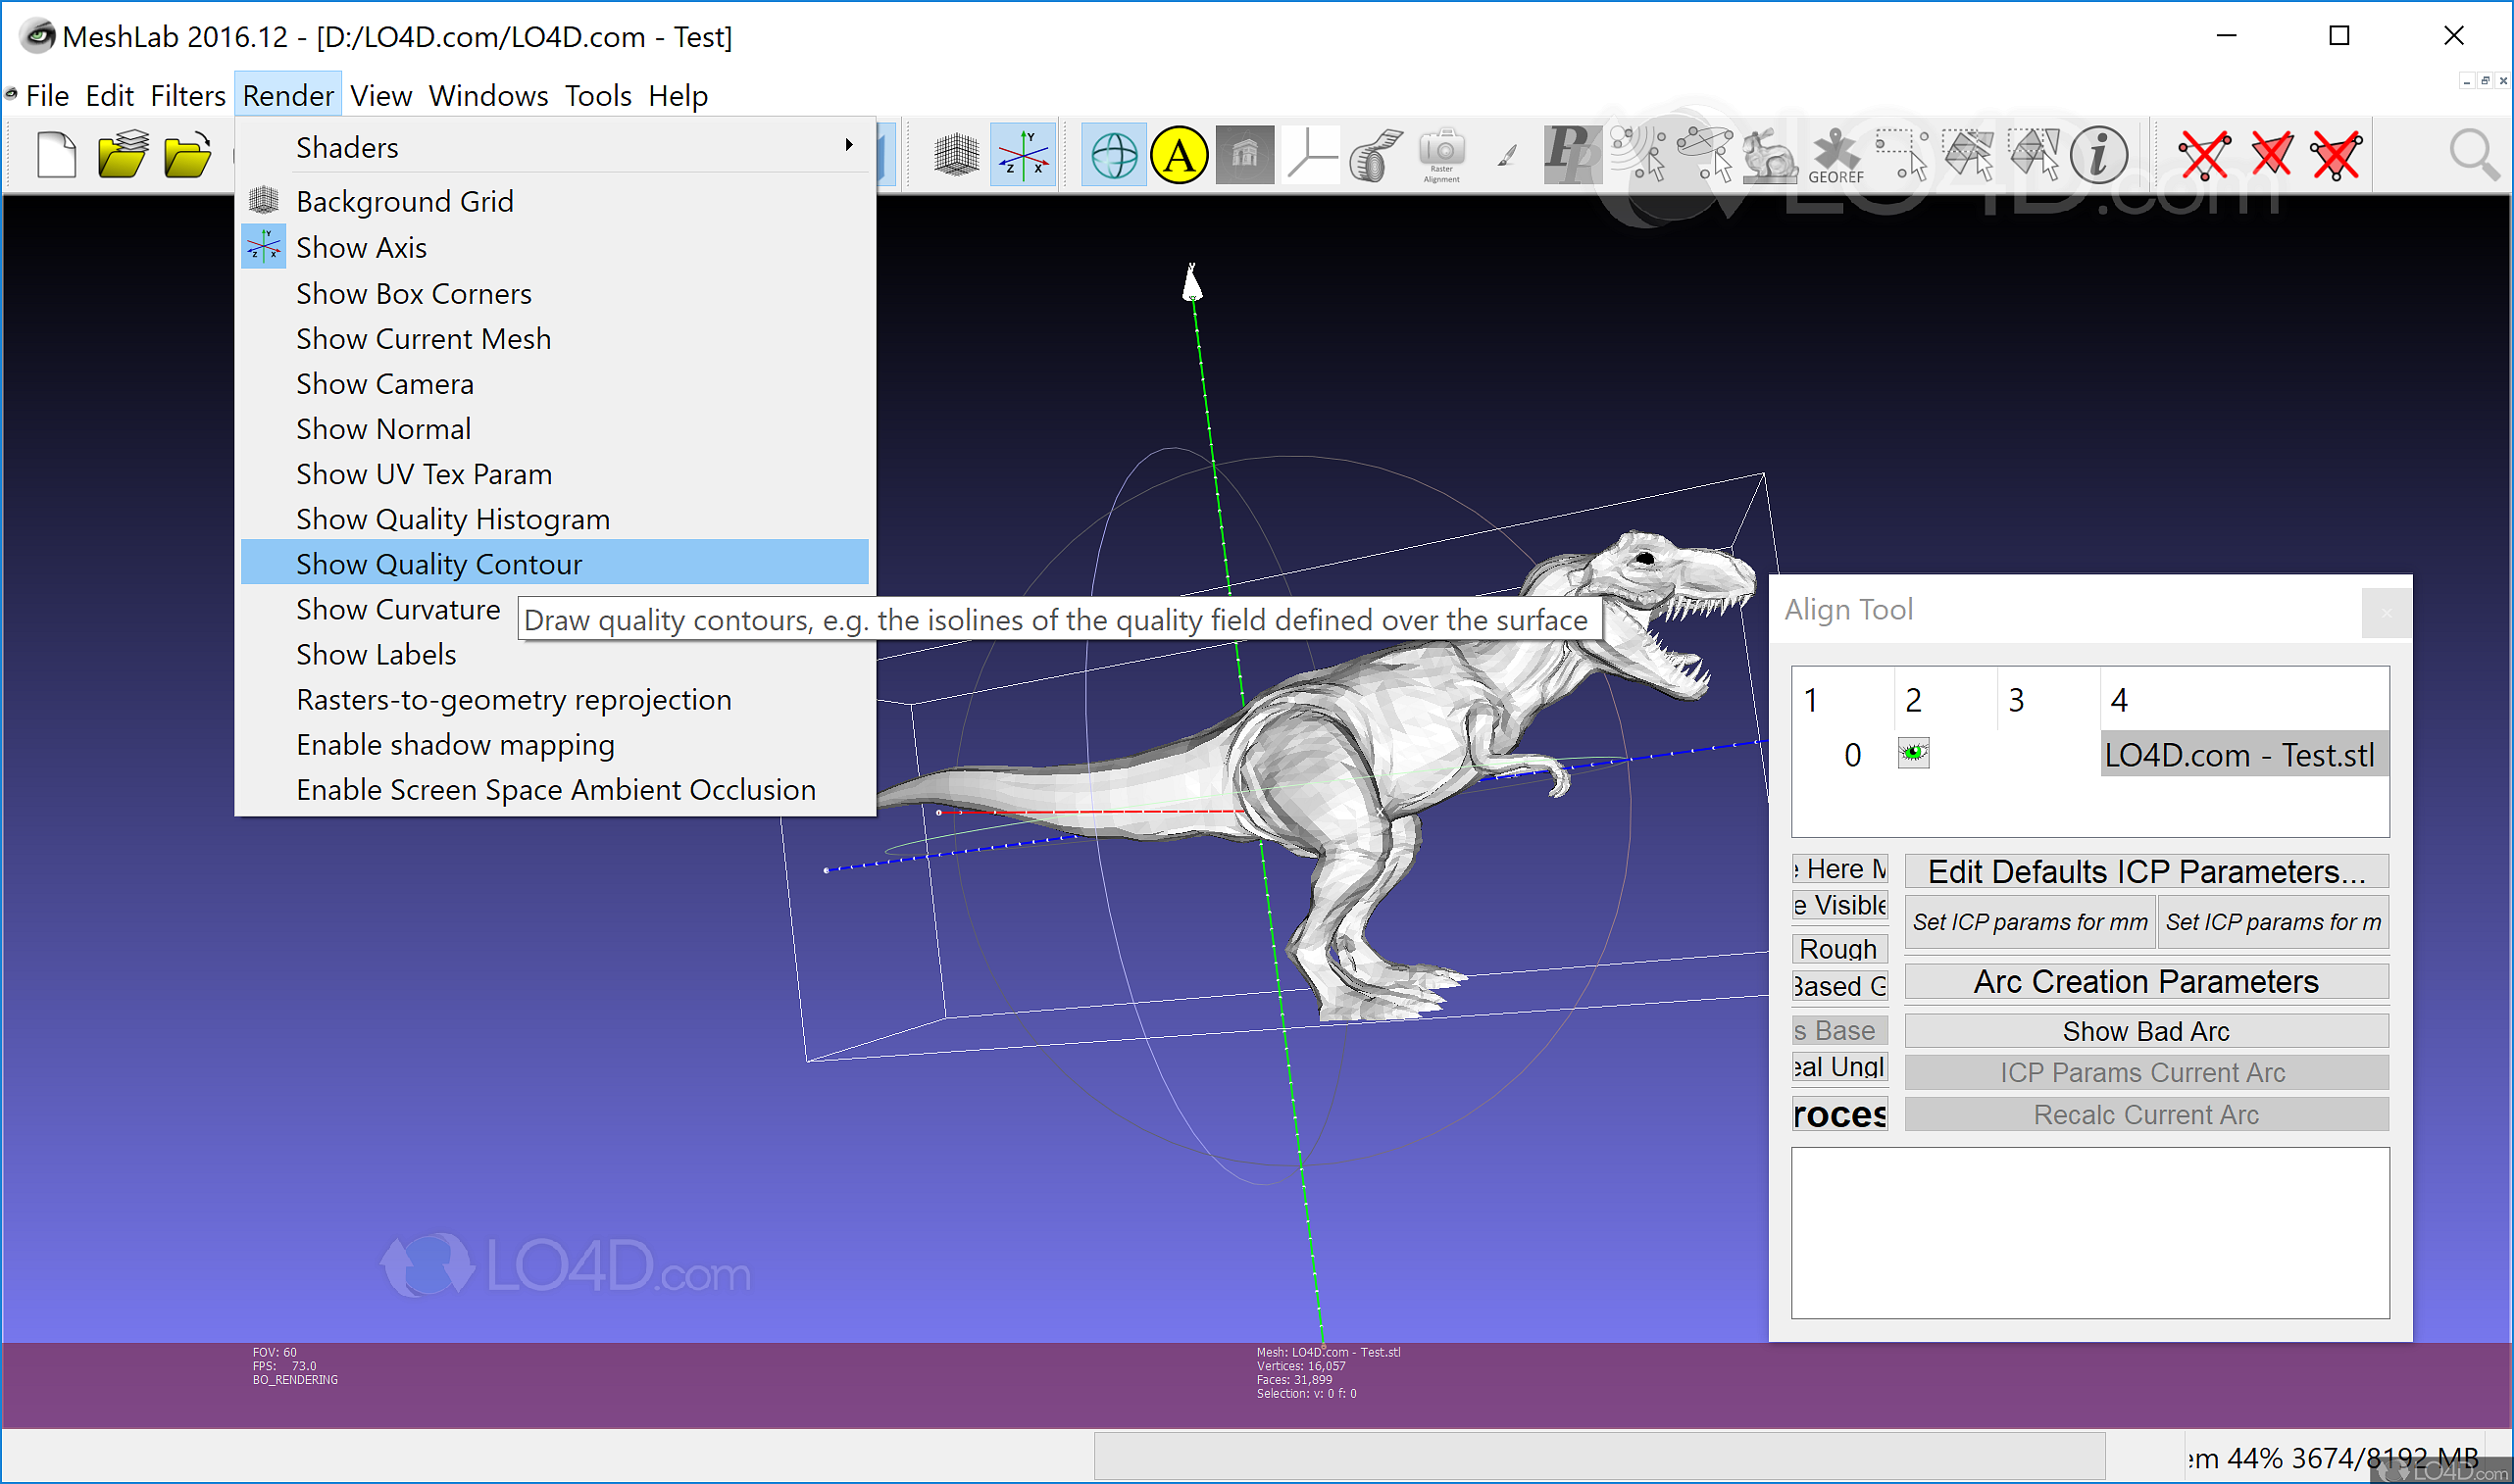
\includegraphics[width=4in]{figures02/meshlab.png}
\caption{MeshLab (view, edit and process).}
\end{center}
%\label{fig2:mypicture3}
\end{figure}


\subsection{FreeCAD}
FreeCAD is a 3D CAD/CAE parametric modeling application. It is primarily made for mechanical design, but also serves all other uses where you need to model 3D objects with precision and control over modeling history \cite{freecad}.

 \begin{figure}[!h]
\begin{center}
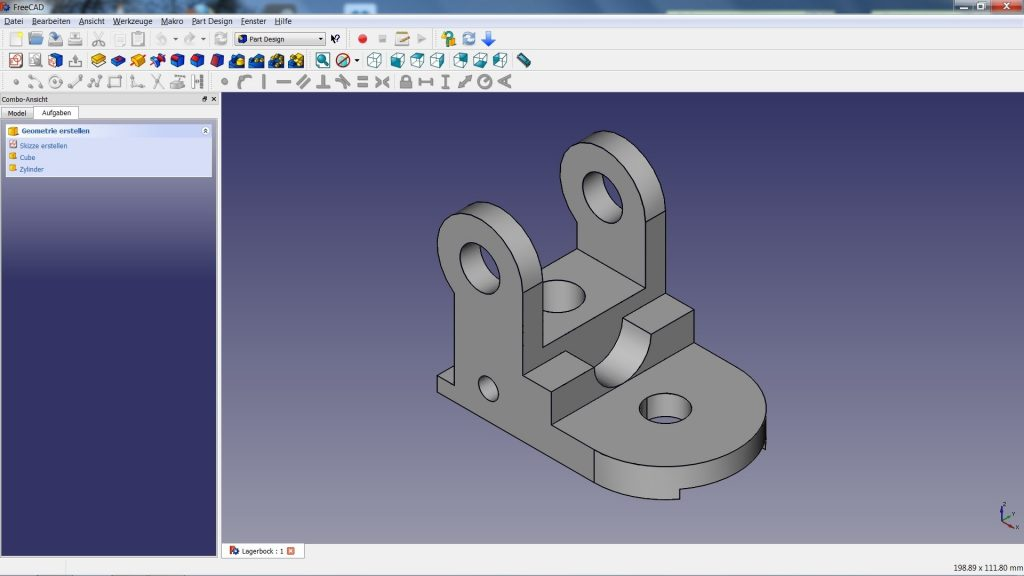
\includegraphics[width=4in]{figures02/freecad.jpg}
\caption{A view of the FreeCAD interface.}
\end{center}
%\label{fig2:mypicture3}
\end{figure}
